\section{Alumnos}
De la sección de los alumnos, se analizaron 41 resultados sobre el uso de la aplicación móvil, tanto para probar el reconocimiento, como para ver el listado de los ETS existentes. 
Los resultados, en su mayor parte, son comentarios positivos, sin embargo, a lo largo del desarrollo de las pruebas salieron a relucir varios puntos de mejora sobre la aplicación, en su mayor parte de visualización.

A continuación se detalla el análisis completo:
\subsection{Facilidad de uso del escaneo del código QR}
\begin{itemize}
	\item \textbf{Facilidad de escaneo:} 
	El 60\% de los usuarios calificó la experiencia como \textbf{Muy fácil} y el 33.3\% como \textbf{Fácil} (gráfica~\ref{fig:facilidad-escaneo}). 
	Solo un 6.7\% \textbf{Muy difícil} reportó problemas técnicos, donde la aplicación tardó 10 segundos en detectar el QR (de acuerdo con el comentario del usuario, por baja iluminación en su entorno).
	
	\begin{figure}
		\centering
		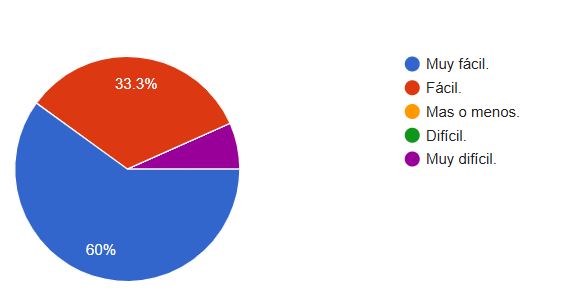
\includegraphics[width=0.7\textwidth]{images/grafico_escaneo.png}
		\caption{Distribución de respuestas sobre la facilidad de escaneo del código QR.}
		\label{fig:facilidad-escaneo}
	\end{figure}
	
	\item \textbf{Tiempo de lectura del QR:}  
	El 46.7\% de los usuarios (7/15) reportó un tiempo de escaneo de 5 segundos, mientras que el 33.3\% (5/15) observó 2 segundos y el 20\% (3/15) tardó 10 segundos (gráfica~\ref{fig:tiempo-escaneo}).  
	Aunque el 80\% de los casos se resolvió en 5 segundos, los tiempos mayores (10s) sugieren la necesidad de optimizar el procesamiento en dispositivos antiguos o con baja iluminación, así como la conexión a internet.
	
	\begin{figure}
		\centering
		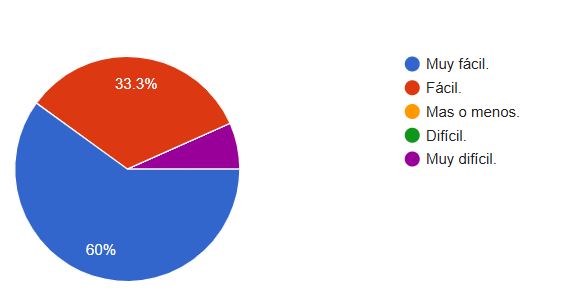
\includegraphics[width=0.7\textwidth]{images/grafico_escaneo.png}
		\caption{Distribución de respuestas sobre el tiempo de escaneo del código QR.}
		\label{fig:tiempo-escaneo}
	\end{figure}
	
	\item \textbf{Precisión del escaneo QR:} 
	La aplicación funciona correctamente en la mayoría de los casos, con 13 de 15 usuarios (87\%) calificando su precisión como buena o excelente (4-5 puntos de 5). 
	
	Solo 2 usuarios reportaron dificultades ocasionales, como que \textbf{la cámara no reconocía el código inmediatamente}. Esto indica que, aunque el sistema es confiable, existen oportunidades para hacer el proceso aún más consistente para todos los usuarios.
\end{itemize}

\subsection{Visualización de la información}
\textbf{Legibilidad de la información:} 
La mayoría de los usuarios calificaron positivamente la claridad de la información (4-5 puntos en una escala de 5), lo que demuestra que el diseño general es efectivo.
Sin embargo, varios usuarios reportaron problemas específicos con la visualización completa de los datos, comentando que: \textbf{los datos de la credencial del alumno no se muestran completos} y \textbf{la información aparece cortada}. Estos comentarios señalan la necesidad de ajustar el formato de visualización de la credencial del alumno para garantizar que toda la información sea visible.